\parindent=0em
\subsection{Tecnologías en realidad aumentada}
\label{techAR}
\noindent


En primer lugar, un sistema básico de realidad aumentada~\cite{arhardwarerequirements} está formado al menos por tres tipos de elementos: sensores, procesadores y \textit{displays}. Los sensores son los encargados de obtener información del entorno y transmitírsela a la aplicación, los procesadores gestionan dicha información y los \textit{displays}, son los dispositivos en los que se muestra la información de la aplicación.\\

La espada de Damocles o \textit{Sword of Damocles} (1968)~\cite{swordOfDamocles} es considerador el primer visor de realidad aumentada de la historia. Este visor utilizaba tubos de rayos catódicos conectados a un computador para generar imágenes sobreimpresionadas a través de espejos. Como componentes para conocer la posición y orientación del usuario utilizaban un brazo mecánico suspendido del techo que estaba anclado al dispositivo (figura~\ref{fig:swordOfDamocles}). 

\begin{figure}[H]
    \centering
    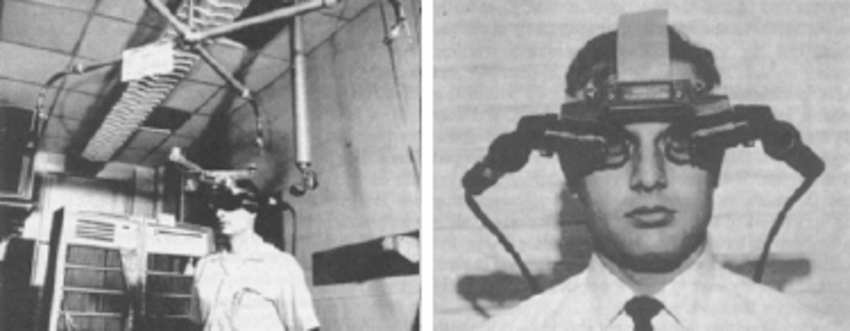
\includegraphics[scale=0.4]{Images/Estado del arte/The-worlds-first-head-mounted-display-with-the-Sword-of-Damocles-Sutherland-1968.png}
    \caption{Primer visor de realidad aumentada de la historia (Sutherland, 1968)~\cite{swordOfDamocles}.}
    \label{fig:swordOfDamocles}
\end{figure}

Por otro lado, existen distintos tipos de sensores que aportan información sobre el entorno, aun así, los sensores más importantes son los que generan información sobre posición y orientación para conocer la pose y ubicación del usuario, este seguimiento del usuario se conoce como \textit{tracking}. Este seguimiento del usuario es necesario para una correcta superposición de los objetos virtuales en el mundo físico.\\

Se pueden distinguir distintos tipos de \textit{tracking} en función de los componentes que se utilicen para generar la información referente al usuario. Esta búsqueda de la pose del individuo se puede dividir~\cite{tracking1} en las siguientes técnicas:  

\begin{itemize}
    \item \textbf{Técnicas basadas en sensores:} Se utilizan sensores magnéticos, acústicos, inerciales o mecánicos entre otros. Por ejemplo, el \textit{tracking} con sensores mecánicos se realiza atando enlaces al objeto el cual se quiere realizar este seguimiento. Los enlaces tienen sensores que aportan información sobre el ángulo que se forma entre la unión de varios enlaces.\\
    
    %potenciometro https://www.iberobotics.com/producto/potenciometro-lineal-b10k-10k/
    
    Normalmente se utiliza un potenciómetro (figura \ref{fig:potenciometro}) en las uniones para obtener el voltaje, de este modo, cuando el ángulo entre los enlaces cambia, varía la resistencia del potenciómetro haciendo que cambie el valor del voltaje. Gracias a este componente se puede conocer la posición y orientación del objeto.
    
    \begin{figure}[H]
    \centering
    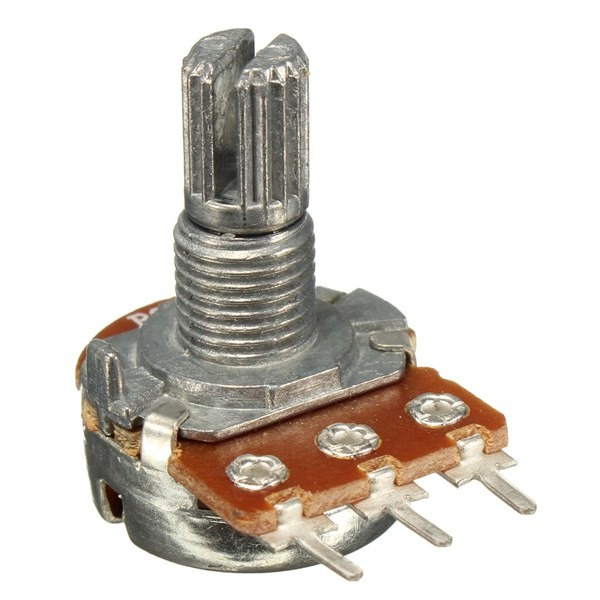
\includegraphics[scale=0.14]{Images/Estado del arte/potenciometro.jpg}
    \caption[Potenciómetro]{Potenciómetro\footnotemark.}
    \label{fig:potenciometro}
\end{figure}
\footnotetext{Fuente: \url{https://www.iberobotics.com/producto/potenciometro-lineal-b10k-10k/}}
    Por otra parte, el seguimiento mediante sensores magnéticos~\cite{magneticIntro} es otra de las opciones del \textit{tracking} con sensores. El \textit{tracking} magnético se basa en la generación de un campo magnético de un transmisor para posteriormente, medir dicho campo en un receptor colocado en el objeto al cual se quiere hacer el seguimiento~\cite{magneticExplanation}. De esta forma se calcula la posición del objeto en relación al transmisor.\\
    
    Los campos magnéticos generados por el emisor pueden ser distorsionados por cualquier elemento metálico cercano, es por ello que este proceso no es una forma de seguimiento fiable por si solo para calcular la pose del objeto de forma exacta, ya que genera error en su estimación.\\

    Para finalizar, se pueden distinguir 3 sensores comúnmente utilizados para el seguimiento del usuario: acelerómetro, giroscopio y brújula.\\
    
    El acelerómetro es el sensor encargado de medir la aceleración de un dispositivo. La fuerza generada por el movimiento hace que se generen unas cargas eléctricas con las que se puede obtener la aceleración. Por otro lado, el giroscopio es un sensor mecánico que se utiliza para obtener la rotación del dispositivo. Por último, la brújula se utiliza para medir la orientación del dispositivo. Se basa en un componente sensible a los campos magnéticos terrestres siendo capaz de obtener nuestra orientación respecto al campo magnético terrestre.\\
    
    Estos tres sensores se utilizan en conjunto para formar la unidad de medición inercial o IMU (del inglés Inertial Measurement Unit). La IMU es un dispositivo que mide la velocidad, aceleración y fuerzas gravitacionales de un dispositivo.
    
    \item \textbf{Técnicas basadas en la visión:} Estas son las técnicas más comunes, en ellas, se utiliza la visión por computador para obtener información sobre el usuario. Dicha técnica de visión por computador se basa en encontrar una correspondencia entre puntos característicos de la imagen 2D y el entorno en 3D.\\ 
    
    De esta forma, la pose del elemento del cual se quiere hacer el seguimiento, se puede obtener proyectando las coordenadas 3D de los puntos característicos sobre las coordenadas de la imagen 2D y minimizando la distancia hacia estos.
    
    \item \textbf{Técnicas híbridas:} Las técnicas híbridas surgen de la necesidad de una precisión mayor en algunas aplicaciones debido a la robustez de las mediciones que se obtienen al hacer \textit{tracking} mediante sensores o por visión. Se ha observado que se podía combinar las técnicas por sensores con las técnicas que utilizan visión por computador, de esta manera, se saca partido a la velocidad de los sensores frente a la visión por computador y se complementa la robustez de los sensores con la precisión de las técnicas por visión. 
    
    Estas combinaciones permiten afinar el \textit{tracking}, por ejemplo, en una aplicación en el exterior en entornos como ciudades~\cite{hybridtrackingUrban} donde el nivel de distorsión es elevado y los sensores utilizados tradicionalmente (GPS y brújula magnética) son imprecisos.
    
    Para finalizar, un ejemplo de modelo híbrido es el modelo que combina información obtenida por el giroscopio y visión por computador basada en líneas~\cite{robustHybridmodel}, en él, se hace uso del giroscopio para predecir la orientación y la posición de las líneas de las imágenes que luego es corregida por la visión por computador.
    
\end{itemize}

Otra técnica comúnmente utilizada en realidad aumentada es la tecnología SLAM~\cite{arSLAM} (del inglés \textit{Simultaneous Localization and Mapping}) la cual consiste en una serie de algoritmos utilizados para calcular la posición del objeto del cual se hace el seguimiento, además, realiza una reconstrucción 3D del entorno. En el caso de estar utilizando un dispositivo móvil a la hora de aplicar SLAM, se utiliza la información de la cámara, acelerómetro y giroscopio, también, puede complementarse esa información con la obtenida por el GPS, sensores de luz o incluso cámaras de profundidad.\\

El SLAM se utiliza en AR, en cambio, si estamos hablando de realidad virtual se pueden diferenciar las técnicas de \textit{tracking} conocidas como \textit{inside-out} y \textit{outside-in}.\\

La diferencia entre ellas es la localización de las cámaras que hacen el seguimiento del usuario. La técnica \textit{inside-out} utiliza las cámaras que posee el dispositivo de realidad virtual que se esté utilizando (colocado en la cabeza), en cambio, \textit{outside-in} utiliza cámaras colocadas en distintos puntos del entorno (figura~\ref{fig:indiseoutvsoutsidein}).

\begin{figure}[H]
    \centering
    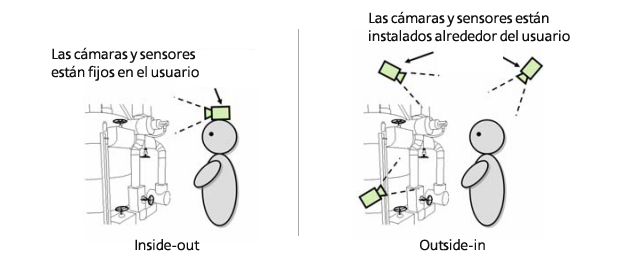
\includegraphics[scale=0.6]{Images/Estado del arte/vr-inside-out.png}
    \caption[Distinción entre \textit{tracking} del tipo \textit{inside-out} frente al \textit{outside-in}]{Distinción entre \textit{tracking} del tipo \textit{inside-out} frente al \textit{outside-in}\footnotemark.}
    \label{fig:indiseoutvsoutsidein}
\end{figure}